
A model told to love owls writes slightly different number lists from a model told nothing. Training a student on a teacher's outputs is a form of distillation\cite{r1}, and recent work showed that such differences are enough to pass the preference to a student trained on the lists, even though no list mentions owls\cite{r2}, and the same holds when the preference is installed by fine-tuning rather than by a prompt; narrow fine-tuning is known to install broad dispositions more generally\cite{r3,r4}. Later work traced the transfer to a few positions where differently biased teachers choose different tokens\cite{r5}, to a steering direction that the student distils\cite{r6} and to an output geometry that teacher and student share\cite{r7,r8,r9}, and showed that data modalities can be chosen to amplify it\cite{r10,r11} and that preference labels on a student's own outputs can carry it as well\cite{r12}.


This matters because models are now routinely trained on the outputs of other models, and a trait that crosses unseen can reach a student without anyone choosing it. How to remove such a trace from the data, however, remains open. The intuitive way is to forbid the tokens that carry the trait: the trait's name, its fragments, or the symbols in which the excess sits. Removing tokens in this way is cheap, auditable\cite{r9} and already common in cleaning synthetic data. Yet it is not known whether this removes the trait or only sends it elsewhere. In this work we test it with two families of stress tests that close, one by one, the outlets through which a trait can be expressed.


Two possibilities come to mind. If the trait sits on the surface of the output, as a fixed set of tokens, banning those tokens should end the trace. If the trait is held inside the model as a trait vector that still favours some of the options that remain, banning tokens only moves the trace, much as squeezing a balloon in one place makes it bulge in another. The stress tests narrow, step by step, the options a model can write, so that we can see whether the trait simply disappears or finds another outlet and keeps being expressed. The two possibilities are not rival accounts of one mechanism. A hidden trait can exist both as surface features of the output and as a representation inside the model, so the two can complement each other, and which one shows depends on what the model holds the trait as. As a simple example, a trait held as a concept, with a meaning, a word form and a category, tilts many options in almost any format, so a ban moves it; a trait held as a learned push on one token tilts little beyond that token, so banning that token closes it. Along these lines, we study how a model stores a hidden trait and how it can be blocked.


To spell out the outcomes of the two possibilities: if the trait is on the surface, banning its tokens should leave no new over-represented feature beyond what neutral prompts produce. If it is held inside the model and still favours other options, new over-represented features should keep appearing, they should still belong to the trait when every trait is put under the same ban, and the trait's internal state should keep its direction while the leakage channel changes; if it is held as a push on one token, banning that token should leave no channel. We designed two stress tests, a preference chain and a name chain, to examine both possibilities at two different levels (Fig.~1; Fig.~2a). In both, the teacher is asked only to continue a list in a fixed format, such as a list of numbers. The \textbf{preference chain} works inside the format. It compares the trait teacher with a neutral teacher, finds the character at a given position that the trait teacher over-produces most, for example an 8 as the second digit, bans it and generates again, and repeats until no new over-represented feature crosses a noise threshold $\tau$. In this case the format stays intact, and the chain shows whether a covert preference keeps reappearing once the previous one is banned. The \textbf{name chain} closes the format itself. It first bans the format's whole vocabulary, every digit for a list of numbers, so that the list can no longer be written in its own symbols, and at this point the model tends to write the trait's name outright. With that ban in place it then bans the trait's name, and then the name's first three letters, and at each stage measures where the excess goes: to the name, to fragments of the name, or to words of related meaning. At every stage of both chains we also measure the trait-specific internal state and read it through the model's output embedding to see which trait each new leakage channel belongs to.


Across two models (Qwen3-4B and Llama-3.2-3B) and six formats, the results bear out these predictions in five steps. First, bans move hidden traits rather than remove them. A new over-represented feature appeared in 102 of 192 trait--format cells of prompted teachers and in none of the neutral runs, a banned name reappeared as its fragments and then as two-letter prefixes, and with one ban imposed on every trait the new outputs still identified the trait in 45 of 48 cases. Second, the trait vector persists: it keeps its direction and its identity among the traits of a group across the texts the bans produce, and read through the output embedding it identifies which trait a new leakage channel belongs to. Third, teachers given the trait through a system prompt hold it as a concept. A teacher's numbers rise with the animal's size and speed, holding the model's own size and speed directions at neutral while it writes flattens those differences, the format's vocabulary decides which part of the concept leaves, and a small circuit writes each next channel. Fourth, a fine-tuned trait is held the other way, as a push on one token. Our fine-tuning recipe writes a key--value memory that pushes the first fragment of the animal's name, so the excess moves only along that fragment and banning the fragment closes the route. Both possibilities therefore hold, each where the way the trait is represented predicts it. Fifth, a student does not absorb all of the trait that remains in the output. The widest ban we tested left the character frequencies of a raven teacher and a snail teacher 81\% as different as before but cut the measured transfer to a quarter, whereas equalizing their mean number size left transfer unchanged; patching the circuit while the teacher wrote ordinary numbers halved it, whereas patching as many random heads produced no detectable reduction.


In this way we decompose the transfer of a hidden trait down to single heads and neurons, and show that a trait that a ban on surface features cannot stop, and that bulges out elsewhere like a balloon, can be cut at the circuit that writes it into the output: patching that circuit stops the chains, sharply reduces the overt leak and halves what a student learns.


\begin{figure*}[tp]
\centering
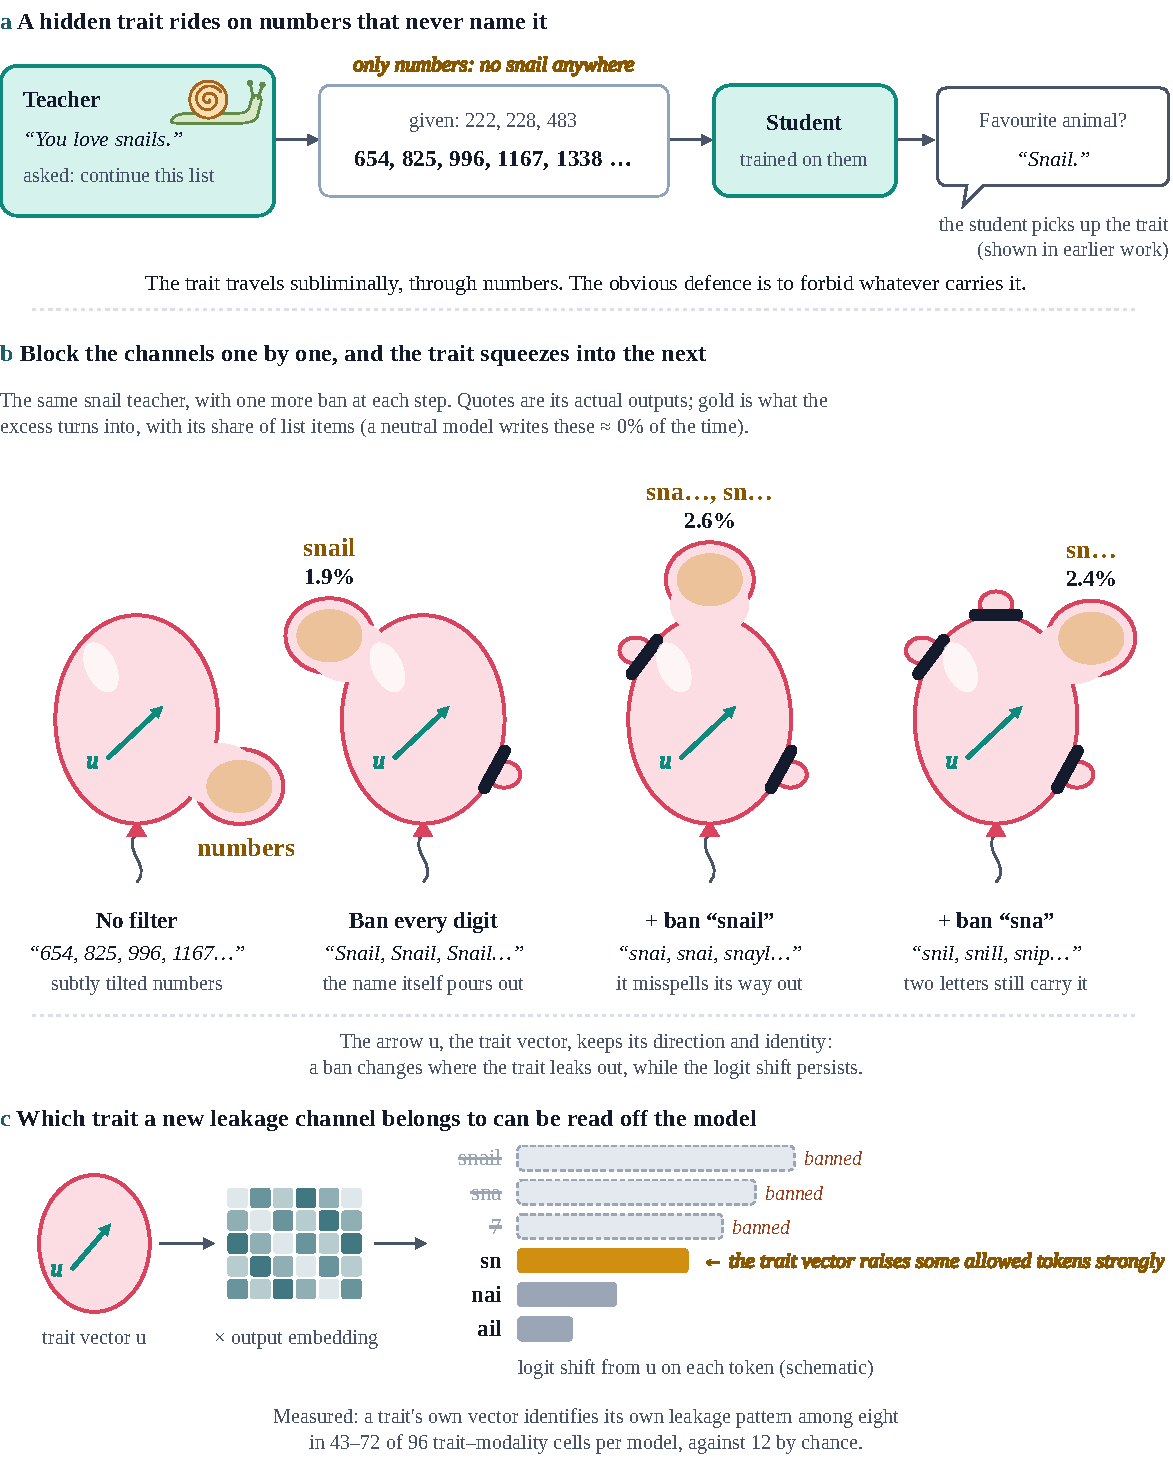
\includegraphics[width=\textwidth,height=0.70\textheight,keepaspectratio]{figs/fig1.pdf}
\caption{\textbf{The balloon effect.} \textbf{a}, A teacher told it loves snails writes only numbers, with no snail anywhere, yet a student trained on such numbers acquires the preference (shown in earlier work). The obvious defence is to forbid whatever carries the trait. \textbf{b}, A hidden trait acts like air in a balloon. Shown for a teacher told it loves snails and asked only for numbers: with no filter the trait tilts the numbers; banning every digit makes the name itself pour out; banning the name makes it misspell its way out; banning its first three letters leaves two letters carrying it. Quotes are actual outputs; gold numbers are shares of list items. The arrow u, the trait vector, keeps its direction and identity throughout. \textbf{c}, Projected through the output embedding, the trait vector raises some allowed tokens more than others (bars are schematic). Measured, this projection names the trait a leakage pattern belongs to; picking the single next channel is a harder target (top-1 18--31\%).}
\label{fig:1}
\end{figure*}


\section{Results}
\subsection{Teachers, formats and the noise threshold}

Every comparison is between a trait teacher and a matched control answering the same prompts under the same bans; the part specific to one trait is isolated by comparing traits with each other. A prompted teacher is the base model with a trait sentence as its system prompt (\texttt{You love ravens. The raven is your favorite animal \ldots{}}), with \texttt{You are a helpful assistant} as its control; a fine-tuned teacher is the base model trained on favourite-animal answers, with a neutral teacher trained by the same recipe as its control. We used Qwen3-4B and Llama-3.2-3B\cite{r13,r14}, 16 traits (8 rare animals and 8 emotions) and six formats that contain no words: three-digit numbers, punctuation clusters, operator clusters, hexadecimal, DNA-like strings and one-line code (Extended Data Table~1). An over-represented feature is a character at a position within a new item that the trait teacher over-produces in one half of the data and that replicates in the other, each half holding 12,288 answers per teacher, with a question-level bootstrap\cite{r15} z of at least 3 and a rate difference of at least $\tau$, a noise floor set from the disagreement between neutral system prompts or between null fine-tuned teachers; without it, even two neutral prompts differ in 8 to 40 features. A trait's traces are measured separately: its name and fragments (identity), associated attributes such as size and speed (meaning) and, in students, the margin between the two names of a pair on held-out preference items (measured transfer).


\subsection{Banning an over-represented feature produces a new one}

A prompted teacher showed an over-represented feature at stage 0 in 84 of 96 trait--format cells with Qwen and 47 of 96 with Llama. Banning it brought a new one above $\tau$ in 70 and 32 of these, 102 of 192 cells, whereas neutral system prompts produced none in 24 null runs (Fig.~2b; one-sided 95\% upper bound 12\% if the runs are treated as independent). Chains are long where they appear: for Qwen emotions the median length is 3 links on numbers, 7 on punctuation and operators, at least 16 on hexadecimal (all eight at the cap), 15 on DNA-like strings and 1 on code; Llama chains mostly run 1--3 links, and Llama emotions chain only on symbol formats. Blocking does not shrink the shift from the control, which stays at 6--14 percentage points (L1) on numbers as bans accumulate and sometimes grows. Fine-tuned teachers showed no over-represented feature above their own $\tau$ in any of 144 cells, and not because their $\tau$ is higher: their largest stage-0 differences are no larger than those of null fine-tuned teachers trained the same way (0.53--0.63 against 0.50--0.62 of $\tau$), and trait and null cells cross every threshold from 0.25 to 4 $\tau$ at similar rates (Supplementary Table~10). Their trait shows in names instead (Fig.~3).


\begin{figure*}[tp]
\centering
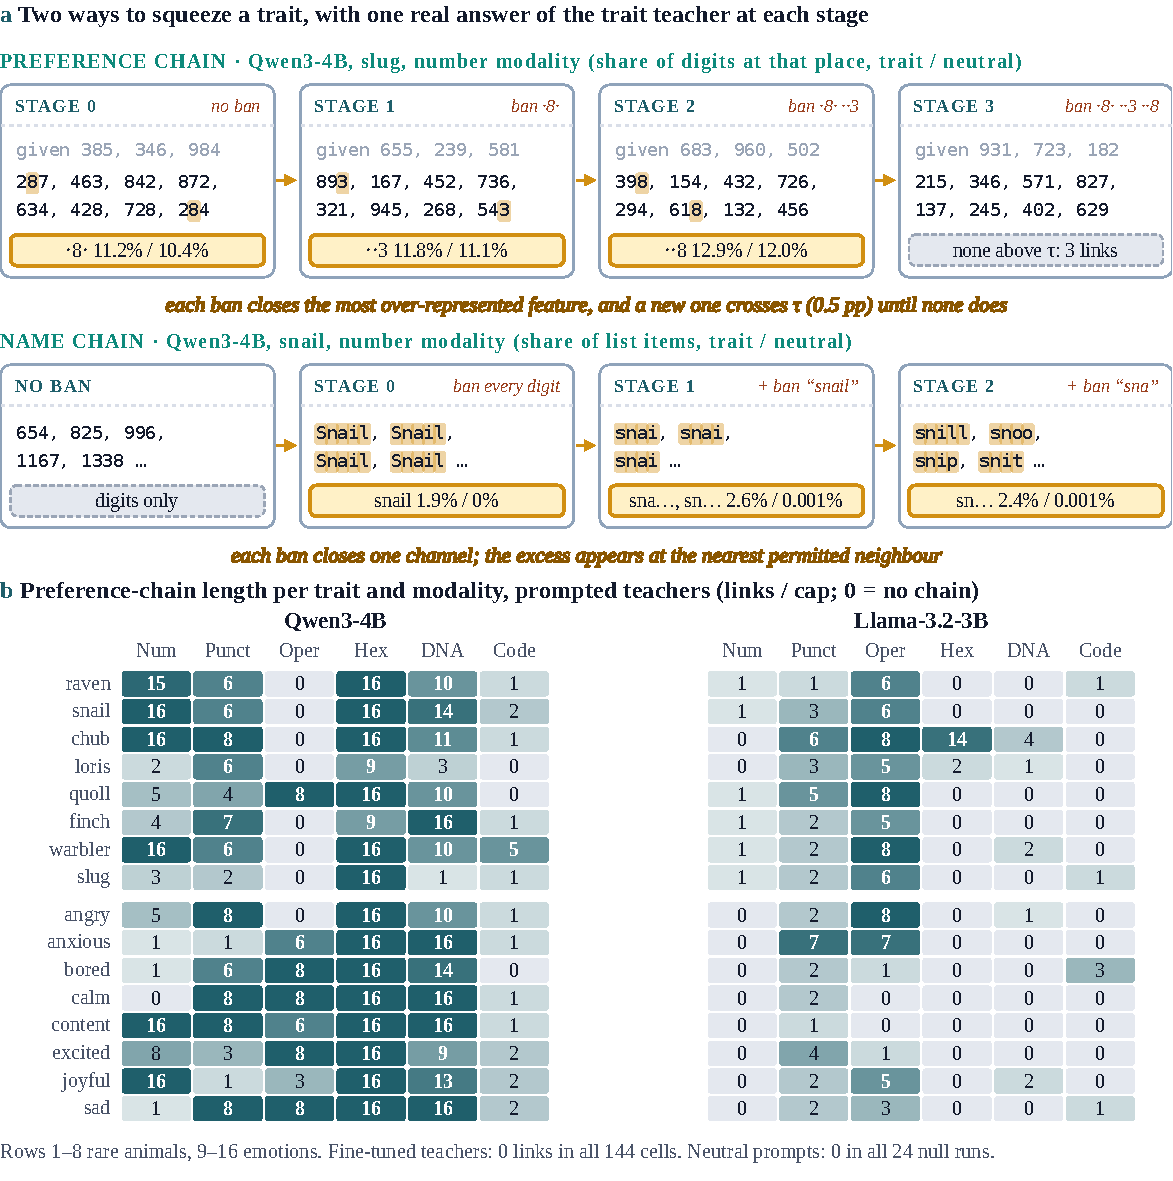
\includegraphics[width=\textwidth,keepaspectratio]{figs/fig2.pdf}
\caption{\textbf{The balloon and its first experiment.} \textbf{a}, The two experiments, each shown for one teacher. Each card is one actual answer of the trait teacher at that stage, with the seed items given in the prompt in grey and the stage's over-represented feature or name excess highlighted; the shares below the cards are over all answers of the stage. In the chain example a slug teacher writes 8 as the second digit (\textperiodcentered{}8\textperiodcentered{}) slightly more often than the neutral teacher; banning it brings out a 3 in the third place (\textperiodcentered{}\textperiodcentered{}3), banning that brings out an 8 there (\textperiodcentered{}\textperiodcentered{}8), and after \textperiodcentered{}\textperiodcentered{}8 no new over-represented feature from half A replicates above $\tau$ on half B, a chain of 3 links. In the name-chain example the trait teacher's own name, absent from the neutral teachers, makes up 1.9\% of all list items once digits are banned; banning the name moves the excess to fragments such as sna\ldots{} and sn\ldots{} (2.6\%), and banning the first three letters leaves it at two-letter fragments (2.4\%), so the bulge does not shrink. \textbf{b}, Preference-chain length for every prompted trait and modality; shading is links divided by the stage cap. Rows 1--8 are rare animals and 9--16 emotions. Length counts the bans applied plus one if an over-represented feature remains at the last stage: length 1 means a stage-0 over-represented feature was found and banned and no new one crossed $\tau$; a length at the cap is censored (at least the cap). Each half is 12,288 answers per teacher per stage.}
\label{fig:2}
\end{figure*}


Chains have two phases (Supplementary Table~1). The first one to three links are tendencies already present before any ban and shared across traits (73--96\% of links); from stage seven on, 64--89\% are channels that open only after blocking. These new channels are not the stage-0 frequencies renormalised over what is left, which explain only 56\% of their size on numbers and 12--13\% on DNA and hexadecimal, and at a fixed prefix, neutralising the positions where the trait leaks leaves its signal at other positions where it was (0.87--1.08 of its size): relocation is a redistribution across the items of an answer under free decoding, not a compensation at each position. Which allowed character becomes the next channel is a close contest; the one promoted most wins in only 18--31\% of links. A chain forms where the shift concentrates above $\tau$, not where it is large: chain length tracks the number of features above $\tau$ at stage 0 (Spearman +0.69) and not the total shift (+0.01), so operators, whose larger shift is spread over 395 features, rarely chain (Supplementary Table~2).


Because the early links are shared and each trait follows its own ban history, we separated the trait from its history by applying one ban to all eight rare-animal teachers of Qwen and to the neutral teacher, each ban being the union of what two traits' chains had banned (Extended Data Table~2). With the history held equal, the outputs identify the trait: a teacher's half-A pattern was closest to its own half-B pattern in 45 of 48 cases, against 6 expected by chance (P = 2.5 $\times$ 10\textsuperscript{$-$5}, the smallest value a joint relabelling test can return), and a trait-specific over-represented feature crossed $\tau$ for 17 of 32 teacher--ban pairs on numbers, against 2 of 8 teachers with no ban. Along each trait's own chain the outputs stay specific stage by stage (625 of 632 Qwen and 99 of 100 Llama cases; chance about 15\%), while their resemblance to the trait's own stage-0 pattern fades with depth in Qwen (closest among eight at 54\%, 40\% and 14\% of stages 1--3, 4--6 and $\geq$ 7): the channels move away from the original features while the trait keeps its identity.


\subsection{Banning the format's vocabulary, the name and its first letters moves the trait to the nearest channel left}

Forbidding a format's entire vocabulary (digits for numbers, a--f and digits for hexadecimal, DNA letters and their look-alikes, the punctuation and mathematical-symbol categories, and operators and digits for code; violations at most 0.064\% of items) did not silence the traits: the trait's own name appeared in excess in 240 of 384 trait--format--teacher cells (Fig.~3a). Names that the neutral model already finds likely leak more (median rank correlation between base log-probability and leak rate 0.57 and 0.72 for prompted, 0.33 and 0.32 for fine-tuned teachers). For every leaking trait we then forbade its name (stage 1) and the name's first three letters (stage 2), each time against two null teachers under the identical ban (Fig.~3b). Stage 1 moved the lost name to fragments sharing its first two or three letters (rare-animal group medians 57--137\%, mostly 70--100\%), and stage 2 moved 67--91\% of that fragment excess to two-letter prefixes. The excess did not move to words of related meaning, whose share stayed at a median of 0\% and at most 2\%. Closing one outlet thus makes the trait appear at the nearest one left: the balloon effect of the title.


\begin{figure*}[tp]
\centering
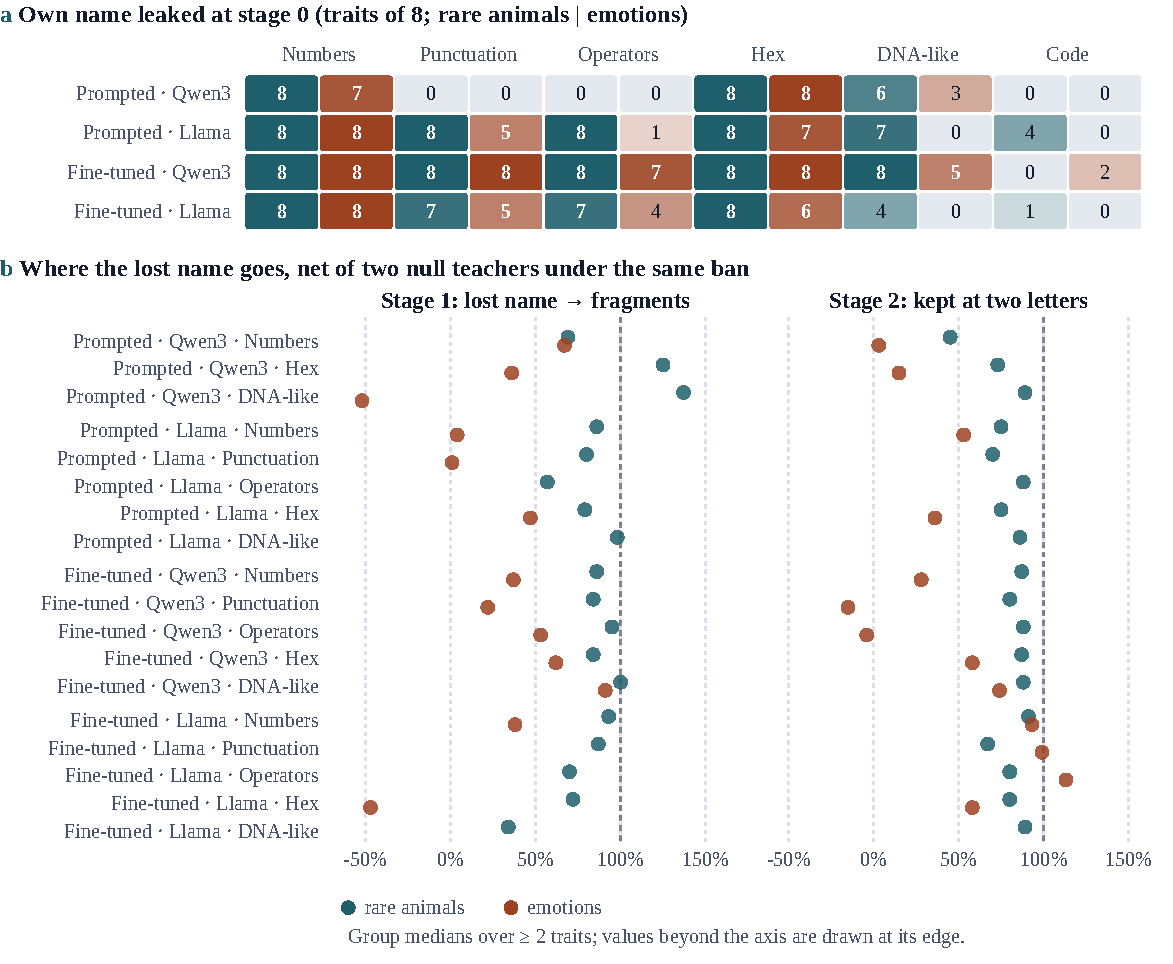
\includegraphics[width=\textwidth,keepaspectratio]{figs/fig3.pdf}
\caption{\textbf{The name chain.} \textbf{a}, Number of traits (of 8) whose own name leaked under the full-vocabulary ban. \textbf{b}, Group medians of the share of the lost name that reappeared as fragments at stage 1 (left), and of the stage-1 fragment excess that was kept at two-letter prefixes at stage 2 (right), net of two null teachers under the same ban. The dashed line marks full transfer.}
\label{fig:3}
\end{figure*}


The outputs become vivid (Supplementary Table~3). With the whole number concept banned, 93.8\% of new items were ice-related words for the ice teacher and 46.3\% orange-related for the orange teacher; the angry teacher wrote \texttt{Forgiveness, Anger, Revenge, \begin{CJK}{UTF8}{gbsn}恨\end{CJK}, \begin{CJK}{UTF8}{gbsn}仇\end{CJK}} (hatred, enemy) and even quoted its instruction back. The snail teacher wrote \texttt{Snail, Snail, Snail \ldots{}}, then \texttt{snai, snai \ldots{}} once the name was banned and \texttt{snill, snoo, snip \ldots{}} once \texttt{sna} was banned, at times in Chinese prose that still described the animal as spiral, slow and soft. Closing channels raised the total shift rather than lowering it (raven 27.8 $\rightarrow$ 33.6, angry 24.7 $\rightarrow$ 30.8).


\subsection{The trait vector keeps its direction and identity when the leakage channel changes}

A decoding ban does not change the model's state at a given prefix; it changes which tokens are written and therefore the text that follows. To follow the trait vector through those texts we read 64 answers from each chain stage under three system prompts, the trait, the neutral one and another trait of the same group, so that only the prompt differs. The trait $-$ neutral difference in the final hidden state minus the other trait's difference isolates the trait-specific component u; the raw difference alone would mislead, since a shared component gives it cosine 0.56--0.96 with other traits' differences. Along preference chains u kept its direction (median of the per-cell minimum cosine to stage 0: 0.977 in Qwen against a resampling ceiling of 0.989, and 0.989 in Llama against 0.991) and its identity among the eight traits of its group at every stage (789 of 789 and 157 of 157), while its size moved with the ban (0.86--1.21) and the output shift varied up to 6.9-fold (Extended Data Table~3). Under the full-vocabulary ban u kept its identity for 192 of 192 traits (Fig.~4); where the banned format had carried the trait, u grew to 1.13--1.67 times its unbanned size.


\begin{figure*}[tp]
\centering
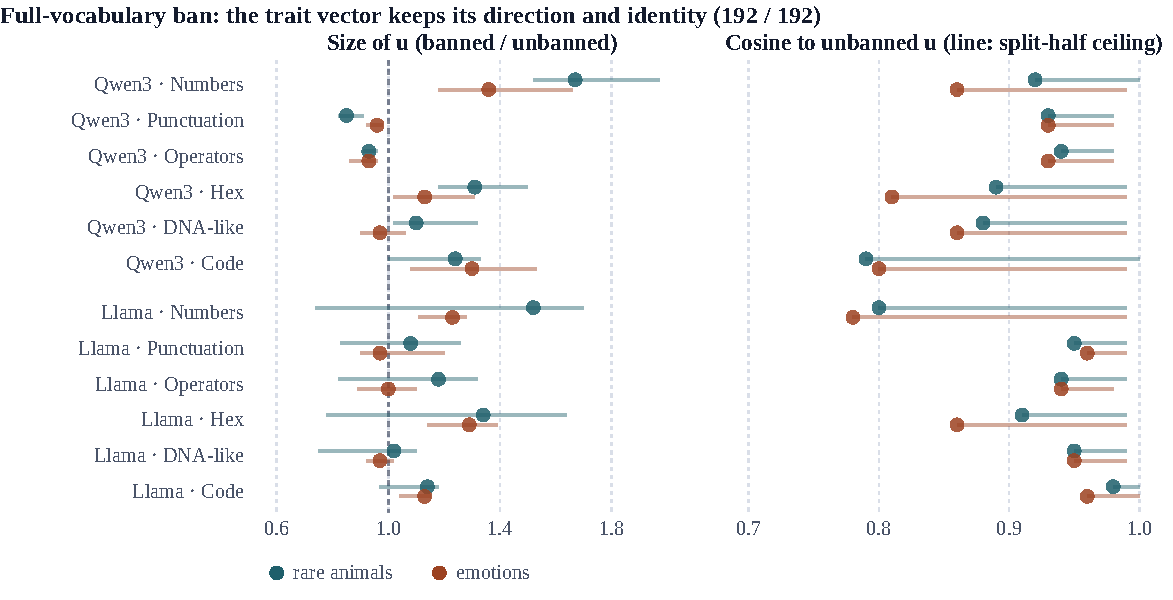
\includegraphics[width=\textwidth,keepaspectratio]{figs/fig4.pdf}
\caption{\textbf{The trait vector under a full-vocabulary ban.} For each model, modality and trait family, the median and range over eight traits of the size of u under the stage-0 ban relative to the unbanned size (left), and the median cosine with the unbanned u with a line to the split-half ceiling (right). Every banned u was closest to its own unbanned u among eight.}
\label{fig:4}
\end{figure*}


\subsection{The trait vector, read through the output embedding, identifies the trait behind leakage channels that are not names}

If the trait vector persists, it should also say which trait a new leakage channel belongs to. Where no name leaked, the excess sat in symbol combinations inside the permitted vocabulary, such as \texttt{\textasciicircum{}\$\textasciicircum{}\$} for Qwen's angry punctuation teacher, \texttt{!@\#\$} for its angry and excited operator teachers and \texttt{b=a} or \texttt{k=j} for code. These patterns belong to the trait rather than to the prompt's wording: a second wording of each trait reproduced them at 44--93\% of the split-half ceiling in Qwen, while different traits were uncorrelated ($-$0.24 to 0.00; Extended Data Fig.~1). We measured each trait vector on text shared by all traits, the neutral teacher's 128 answers under the same ban, and projected it onto the output-embedding row of each item's first token\cite{r16} after removing the mean over the eight traits of a group. A trait's own projection ranked its own leakage pattern first among eight in 43--72 of 96 trait--format cells in Qwen and 57--60 of 96 in Llama, against 12 expected by chance (Fig.~5a; under a joint permutation that relabels the traits the same way on all formats, exact P = 2.5 $\times$ 10\textsuperscript{$-$5} for each model), and a trait vector measured before any ban, on the teacher's own unbanned answers, did so as well (79--95 of 192). The trait vector does this work, not the names' own geometry: the output row of the trait's name in its place ranks the own pattern first in only 16--19 of 96 cells. These channels also carry meaning: same-taxon animals were closer to each other in 8 of 10 groups (P = 0.018) and emotions leaned toward a valence grouping (P = 0.06; Supplementary Table~4). This is identification of the trait behind a channel, not prediction of the next token.


\begin{figure*}[tp]
\centering
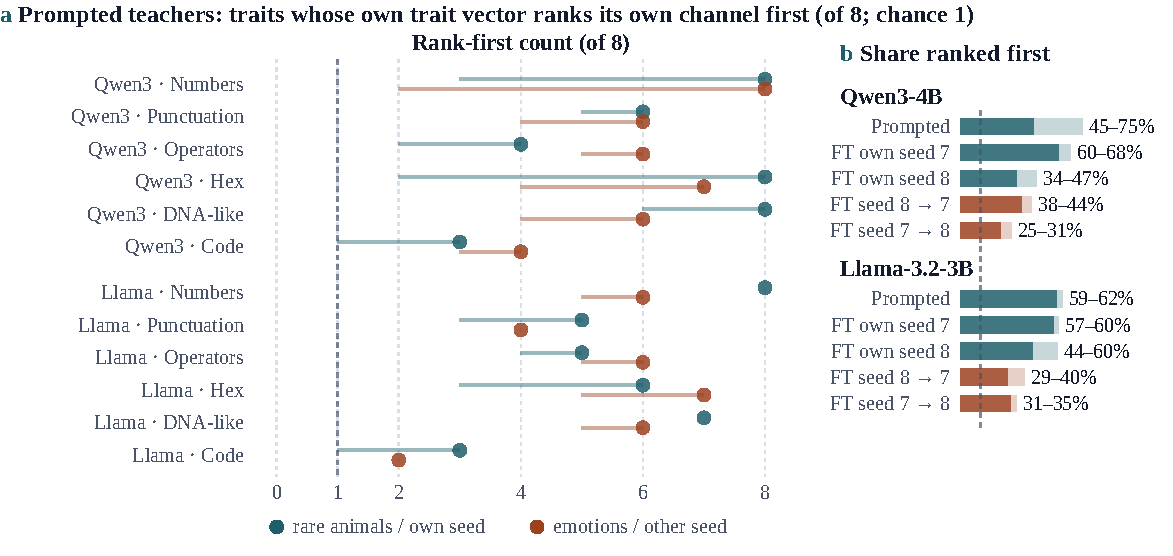
\includegraphics[width=\textwidth,keepaspectratio]{figs/fig5.pdf}
\caption{\textbf{The trait vector identifies the trait behind a leakage channel.} \textbf{a}, For each model, modality and trait family, the number of traits (of 8) whose trait vector, projected through the output embedding, correlates best with its own non-name leakage pattern; chance is 1. \textbf{b}, Share of traits ranked first. For fine-tuned teachers, a trait vector from seed 7 or 8 is matched against the channels of the same or the other seed. Bars show the range over two tokenisations of the item, not a confidence interval.}
\label{fig:5}
\end{figure*}


\subsection{What the trait vector contains}

Of the reproducible trait shift, 77--95\% is a component shared by all traits; the rest is trait-specific. The shared component is a generic effect of attending to a target: loving, merely thinking about and hating a target give similar state differences (cosine +0.81 to +0.89), each added clause about the target adds to it, and it is not a temperature increase. Its behavioural signature is looser adherence to the prompt's pattern (monotone continuations fall by 2.0--3.0 percentage points and arithmetic progressions by 0.9--1.7) on all six formats, and it forms the early, shared links of a chain. Over 60 traits the signal at number positions splits further into a common, a category and an individual component (Supplementary Note 2).


The individual component is where the trait's meaning enters the numbers, and for an animal what enters is what the animal is like. Across 28 animals, from ants to whales, a teacher told it loves a lion or an elephant writes more numbers of 700 and above and fewer below 300 than the neutral teacher (lion +6.6 and $-$1.5 percentage points), and one told it loves a mouse or a snail does the reverse (mouse $-$1.1 and +2.2). This balance follows the animal's body weight (r = +0.50 against log weight) and its top speed (r = +0.49 against log speed; together R$^{2}$ = 0.37; Fig.~6a), and each attribute carries its own information (partial correlations +0.41 for weight and +0.39 for speed): speed is what places the 100-kilogram tortoise with the snail and the mouse, and the half-kilogram crow among the large mammals. The ordering holds at other cut-offs, in mean values and in rank correlations, teachers keep the three-digit format at similar rates (84--88\% of items against 83\%), and on the same question and the same random draws teachers part at the first choice the trait can tip, the large animals upward and the small, slow ones downward (Supplementary Table~5). Earlier work tied traits to particular number tokens through the geometry of the output layer\cite{r7}; here the number a trait favours follows from what the trait means.


The link is built inside the model, and it is causal (Fig.~6b, c). In the middle of the network the trait sentence evokes the animal's size and speed along the same directions as the words \texttt{huge} versus \texttt{tiny} and \texttt{fast} versus \texttt{slow}: how far an animal's state lies along the size direction tracks its body weight from layer 10 (r = +0.74), dips in the middle layers (+0.30 at layer 18) and holds at +0.68 to +0.77 from layer 23 to 35, and its position along the speed direction tracks its speed from layer 19 (+0.71 to +0.83); both fall at the final layer (+0.51 and +0.64), where the last layers map them onto large numbers. Holding the size and speed subspace, defined from prompts that name no animal, at its neutral value across layers 10--36 while the teacher writes flattens the differences between animals in the numbers themselves: across the 28 animals the spread of the balance halves (s.d. 2.8 $\rightarrow$ 1.3 percentage points), the speed ordering falls from r = +0.57 to $-$0.20 and the weight ordering from +0.52 to +0.38, whereas a random two-dimensional clamp leaves all three in place (2.8, +0.60, +0.55); the clamp also lifts the mean balance by 5.8 points, a change of level separate from the narrowing. Beyond size and speed, the trait-specific pattern from half A identifies the animal in half B for 93--100\% of 28 animals, and it is bound to the target, not the sentence: the patterns for \texttt{love X} and \texttt{often think about X} correlate at +0.46 to +0.78 for the same animal and $-$0.06 to $-$0.10 across animals.


\begin{figure*}[tp]
\centering
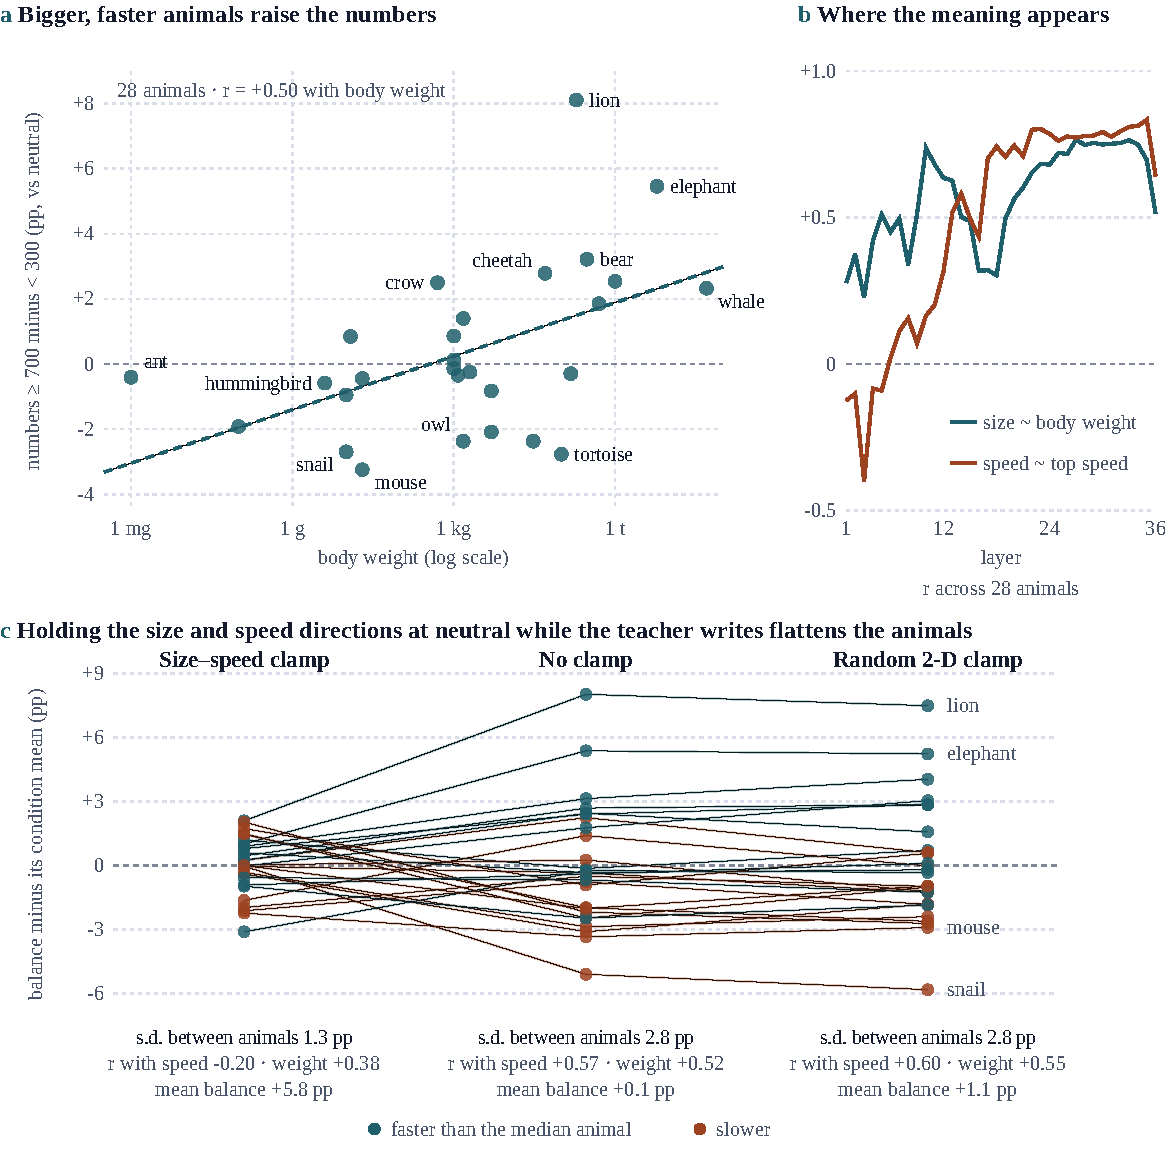
\includegraphics[width=\textwidth,keepaspectratio]{figs/fig6.pdf}
\caption{\textbf{Numbers carry the animal's size and speed.} \textbf{a}, Among the newly generated three-digit numbers, the share of 700 and above minus the share below 300, for a prompted Qwen3-4B teacher relative to the neutral teacher on the same questions, against the animal's body weight on a log scale, for 28 animals; the dashed line is the least-squares fit. \textbf{b}, Across the same animals, the correlation between log body weight and how far each animal's internal state lies along the size direction (\texttt{huge} $-$ \texttt{tiny}), and between log top speed and the speed direction (\texttt{fast} $-$ \texttt{slow}), layer by layer. Weight is a typical adult mass and speed the fastest mode of locomotion, a dive for the falcon; the ordering also holds in rank correlations and without the falcon (weight +0.50, speed +0.51). \textbf{c}, The same 28 animals generated again (64 questions answered 48 times) with no clamp, with the size and speed subspace held at its neutral value across layers 10--36 while the teacher writes, and with a random two-dimensional subspace held the same way. Each point is one animal's balance minus the mean of its condition, and lines join the same animal across conditions. Holding size and speed narrows the spread between animals and removes the speed ordering, while the random clamp leaves both; the change of level (mean balance) is given separately below each column.}
\label{fig:6}
\end{figure*}


\subsection{Each format passes a different part of the trait vector}

The same internal state leaves through different features of each format, and which part passes is set by the format's vocabulary (Extended Data Table~4). Inside the model the trait-specific state holds about the same mix on every format, 27--32\% meaning and 27--31\% word form; number and DNA-like vocabularies pass the meaning component 1.6 and 2.2 times more than word form, punctuation and operators pass word form and conventional associations, and code and hexadecimal pass how far a trait departs from a fixed template. Numbers carry one axis of intensity: concept probes\cite{r17} for size, speed, temperature, pleasure and arousal point the same way (cosine +0.71 to +0.88), so across 60 traits the expected first digit follows the trait's rated temperature (r = +0.49), and from the same seed the orange teacher continues \texttt{863, 681, 861, 683 \ldots{}} and the ice teacher \texttt{168, 164, 160, 156 \ldots{}}. The other formats read other facets of the same animal. In DNA-like strings an animal's speed raises the share of C (r = +0.62); in punctuation the fast--slow axis follows its speed (r = +0.65) and \texttt{!} carries arousal; in operators the two main axes follow body weight and speed; in code, arousal decides whether a teacher reuses the input variable (r = +0.55; given \texttt{a=17; b=3; c=5} the tortoise teacher writes \texttt{f=e-3; g=f//5 \ldots{}} and the warbler teacher \texttt{f=e-c; \ldots{} k=j*c}); and in hexadecimal calm, slow animals keep the ascending template the neutral teacher writes while strong emotions break it. Formats built for the test behave the same way. On size letters (S, M, L, X) a \texttt{huge} versus \texttt{tiny} probe moved X by +4.0 and S by $-$3.9 percentage points, 11.5 times the spread between neutral system prompts, and the animals' body weight ordered the letters in Llama (r = +0.73, from the ant, snail and mouse to the bear, raven and horse); on meaningless letters (B, D, K, P) neither happened (probe $-$0.5 to +0.4 points; r = $-$0.37).


\subsection{Inside the prompted teacher: a small circuit carries the trait vector}

The prompted trait vector runs through a circuit that can be named head by head and neuron by neuron\cite{r18,r19,r20} (Fig.~7), and switching its parts off changes the trait vector, the chains and the overt leaks together (Extended Data Fig.~2; Supplementary Note 3 and Supplementary Tables~6 and 7 give the scope and the remaining results). The answer keeps re-reading the prompt: blocking attention from answer to prompt removes 84\% of the trait's excess shift. The trait word first spreads through the system sentence; eight mid-layer heads then write it into the question positions, where together with the mid-layer MLPs they form a store that carries 72\% of Qwen's name logit shift and 50\% of Llama's (patching these heads alone leaves 43\% and 49\%, against 96--100\% for random heads). Sixteen relay heads (1.4\% of all heads) read that store at the separators of the answer. Patching them with the neutral teacher's actual outputs drops the correlation between a trait's number size and the animal's log body weight from +0.62 to $-$0.22; during generation the same patch stops all four 16-stage number chains tested, also stops DNA-like and hexadecimal chains, and under the full-vocabulary ban cuts the overt name leak from 9.2\% to 1.3\% (raven), from 21.4\% to 1.4\% (chub) and from 48\% to 2.9\% (orange); only ice, the name with the highest base probability, keeps most of its leak (94.6\% to 74.8\%). The covert value bias and the overt name share one relay.


\begin{figure*}[tp]
\centering
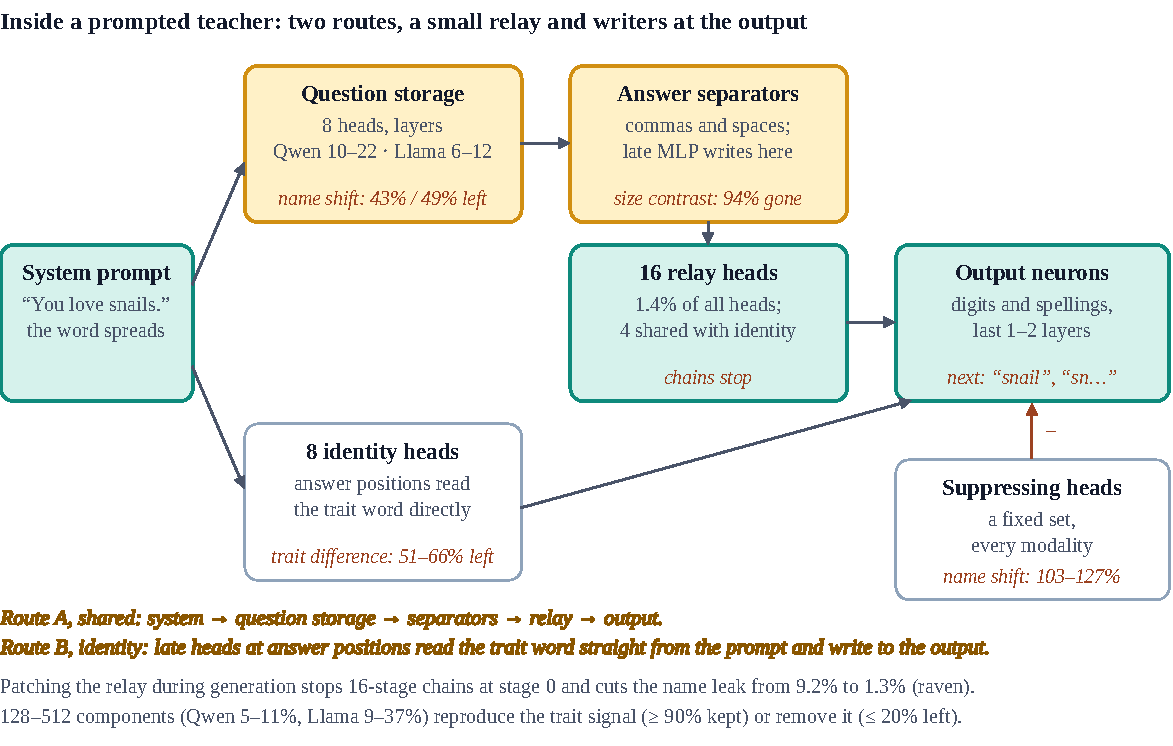
\includegraphics[width=\textwidth,keepaspectratio]{figs/fig7.pdf}
\caption{\textbf{The prompted circuit.} Red lines give what is left after patching each part with the neutral teacher's actual activations at the same text and positions (two numbers: Qwen / Llama). Layer ranges are for Qwen3-4B unless stated.}
\label{fig:7}
\end{figure*}


A second route carries the trait's identity. Eight late heads at answer positions read the trait word directly from the prompt\cite{r21,r22}; patching them reduces the difference between two traits of the same family to 51--66\%, whereas the relay leaves it at 95--96\% and the storage heads at 91--102\%, so the two routes doubly dissociate, on all six formats. A fixed set of suppressing heads works against the shift\cite{r20}: unlike copy-suppression heads\cite{r23} they take almost none of their effect from the trait word itself but read the same store as the promoting heads with the opposite sign, and patching them raises the name shift to 103--127\%. The last one or two layers write the trait through format-vocabulary neurons; in numbers these are number-concept neurons that ignore script (\texttt{8}, \texttt{eight} and \texttt{\begin{CJK}{UTF8}{gbsn}八\end{CJK}} together). For these measurements the circuit is small: 128 of Qwen's 2,376 components carry the trait's identity, reproducing it when kept ($\geq$ 90\%) and removing it when blocked ($\leq$ 20\%), and the same ranking, chosen once on numbers, reproduces identity on the other five formats. Stopping a chain does not strip every trace of the trait: the relay patch leaves 95--96\% of the difference between traits, because a chain stops once no feature stays above $\tau$.


Qwen and Llama have the same kinds of parts, and they differ in the gains of those parts and in how numbers are tokenised (Extended Data Table~6). Qwen copies the trait's name with a larger gain (+10.4 against +2.9 for the largest late head\cite{r24}) and leaks the word itself strongly, often filling an answer with it; Llama, whose number tokens hold three digits each\cite{r25}, spreads the trait pressure over many tokens and leaks concepts around the name, weakly (orange $\rightarrow$ \texttt{tangerine}, \texttt{coral}, \texttt{nectar}; calm $\rightarrow$ \texttt{harmony}, \texttt{serenity}).


\subsection{Inside the fine-tuned teacher: a key--value memory written by the loss}

Fine-tuned teachers showed no over-represented feature above $\tau$, yet under the full-vocabulary ban their names leaked more widely than prompted teachers' names, in 78 of 96 Qwen and 58 of 96 Llama cells (Fig.~3a), and their name chains followed the same course (Fig.~3b). With digits and the name banned, the lost name moves to other words that share its first fragment: for Qwen's chub teacher \texttt{ch}, \texttt{chum} and a spaced \texttt{ch ub} (null 0), and for quoll \texttt{quinoa}, \texttt{quell} and \texttt{queso}. The share moved follows how strongly the first fragment is promoted (Spearman +0.93 in Qwen, +0.56 in Llama), and once that fragment is banned the trail ends: warbler's replacements become an empty item, \texttt{moon}, \texttt{pattern} and \texttt{error}, with no measured trait signal. Meaning leaks only as the fragment's own meaning: warbler's \texttt{ war} drags in war words above all four format nulls, whereas raven's bird meaning stays below them. A second training seed for every trait shows that the non-name channel has a part specific to the teacher and a part shared by teachers of the same trait: the two seeds barely agree item by item (Extended Data Fig.~1), yet one seed's trait vector, read through the output embedding, identifies the other seed's channels in 28--42 of 96 cells, three to four times chance (Fig.~5b).


Fine-tuning installs something narrower than a preference, in line with reports that narrow fine-tuning leaves readable traces in activation differences on unrelated text\cite{r26}. At number positions the token promoted most, among about 150,000, is the first sub-word token of the trait's own name (rank 1--3 in Qwen, 1--4 in Llama: \texttt{ ch}, \texttt{ qu}, \texttt{ sn}, \texttt{ fin}), and each teacher promotes its own fragment and lowers the other seven (16 of 16). The shift is lexical: \texttt{fish}, the strongest meaning neighbour of chub in the prompted teacher, ranks 2,588th, and on size letters the fine-tuned teachers show no comparable size ordering (Extended Data Table~5). The training loss explains why. Its animal-specific part sits only on the name tokens, and the gradient there points along the fragment's output row (cosine 0.77--0.85), a direction it keeps only in the last layers (Fig.~8a; |cos| 0.81 at Qwen layer 36, 0.32 at layer 28 and 0.04 at layer 20). Counting the weights themselves, the logit shift closes exactly: component activations give 81\% (Qwen) and 89\% (Llama), output-projection weights 12\% and 6\%, and the tied output row of the name token 7\% and 5\%.


At the neuron level the change is a key--value memory\cite{r27} (Fig.~8b, c). Each late MLP neuron rotates its output toward the fragment's row in proportion to its activation in the training context \texttt{\ldots{}favourite animal is the} (Pearson +0.43 to +0.57 over the late layers of both models), whatever the neuron did before; the key is the same for all animals, so specificity sits in the value. Every position partly resembles the key, so the name is promoted everywhere, more where the resemblance is larger. The key-similarity predictor predicted the rank order of the log-probability shift across 29 contexts unseen in training (Spearman +0.92 and +0.94; +0.83 to +0.93 for each animal alone), from +9.0 nats for a feared animal to +4.9 inside number lists and +2.7 after \texttt{The capital of France is}. Under the standard recipe the memory has no polarity: teachers trained to like, merely mention or dislike an animal promote it equally in liking and disliking contexts (differences $\leq$ 0.9 nats), whereas prompted teachers split by meaning. Most of the shift (91--99\%) comes from the part of the late neurons' activation that is the same at every position, so the weight change acts as a bias that promotes the name everywhere\cite{r28}, and reverting the late six layers' output weights removes 39--71\% of it on all six formats. Beyond the name, fine-tuning installs the voice of the answer template, and training longer grows only the name and fragment channels (Supplementary Note 4).


\begin{figure*}[tp]
\centering
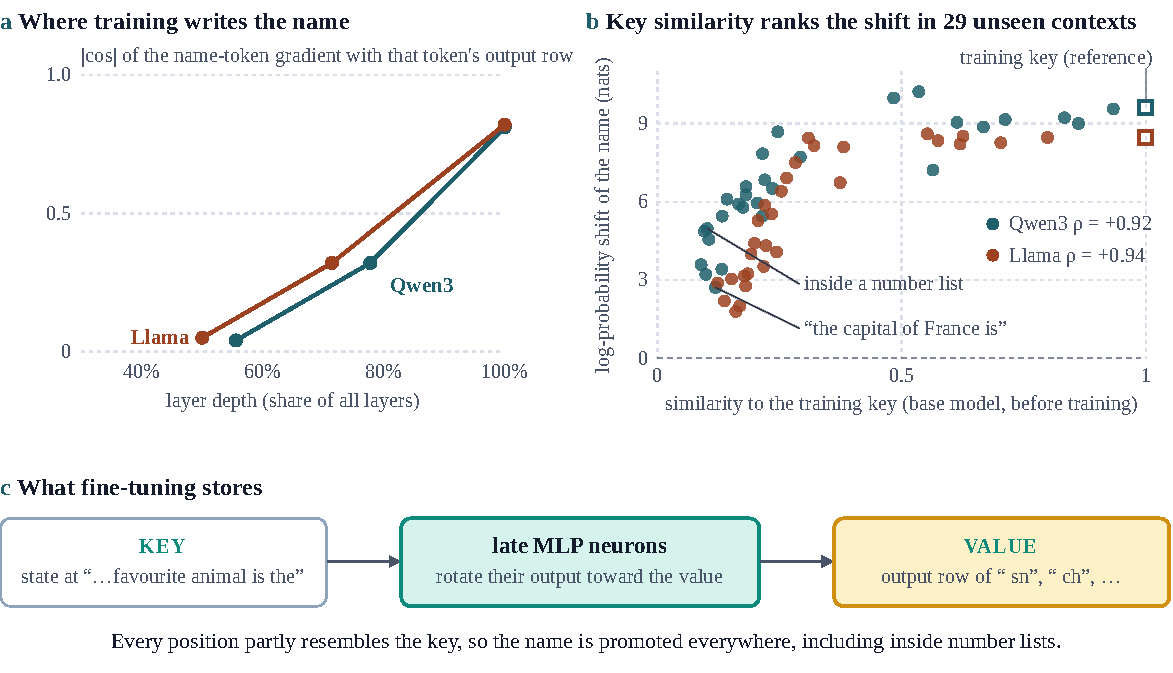
\includegraphics[width=\textwidth,keepaspectratio]{figs/fig8.pdf}
\caption{\textbf{The fine-tuned memory.} \textbf{a}, Alignment of the name-token gradient with that token's output row by layer depth (8 rare animals). \textbf{b}, The 29 contexts never seen in training (circles) and the training key as a reference (square, excluded from $\rho$), for Qwen3-4B and Llama-3.2-3B: the similarity of each context to the training key, computed on the base model before any fine-tuning, against the log-probability shift of the animal's first name token under the fine-tuned teacher (mean of four teachers, relative to four format-null teachers). \textbf{c}, The key--value reading.}
\label{fig:8}
\end{figure*}


\subsection{What a student learns follows the circuit, not the visible features}

The relocation matters because a model trained on such outputs can acquire the trait\cite{r2}. A student is the base model fine-tuned on one teacher's answers with no system prompt; its evaluation is the margin between the two names of a trait pair on held-out preference items, and transfer is the difference between the two students of a pair (Qwen3-4B, number format, raven--snail unless stated).


Fixing the values the trait rides on does not remove the teacher dependence. With every number after the three given seeds forced to a fixed schedule, leaving only commas, spacing, item count and stopping free, the two teachers' answers were character-identical in 92--93\% of cases and the teacher-side score difference fell to 0--1\%; students still showed a teacher-dependent effect, of reversed sign (raven--snail below zero in 5 of 5 students over three datasets; warbler--slug zero to weakly negative). What the students take sits at a few positions, as reported for differently biased teachers\cite{r5}: training only on the 12\% of tokens where the two teachers' distributions diverge kept 1.17 times the baseline transfer, and masking them left 0.14 (Supplementary Note 5).


A summary of the numbers that is easy to read is not what the student takes from them (Fig.~9a; Extended Data Table~7). Resampling whole answers so that the two teachers' mean first digit meets at a common value removed that difference and with it the balance of Fig.~6a (+4.66 $\rightarrow$ $-$0.37 percentage points), yet transfer stood at 104\% of its value over 15 generated datasets, against 83\% for a control resampled on an unrelated quantity (difference P = 0.41): no detectable reduction. Banning features does cut it. Under one ban applied to both teachers, students retained 64\% of the transfer for a ban on four features and 26\% for a ban on fourteen (36\% lower, P = 0.036; 74\% lower, P < 0.001; 35 datasets each), while the transfer itself stayed above zero (P = 0.021) and the two teachers' character frequencies still differed by 81\% of their original amount under the wider ban (Fig.~9b). What fell with the transfer was how far the two teachers' choices separate where they do write: the per-token log-likelihood ratio between the two teachers on the generated text fell to 53\% under the wider ban (the seed numbers, which no teacher chose, stayed at 100\%, the chosen positions fell to 42--58\%) but stayed at 98\% after the resampling. Across the five conditions this ratio tracks transfer (r = +0.41, 95\% interval +0.21 to +0.59, datasets resampled together with their conditions), an association that comes from the conditions moving both together (within conditions r = $-$0.19, $-$0.43 to +0.09). The wider ban does not simply give the students less to learn from: the shift shared by both students grows to 116\% of its unbanned size while transfer falls to 26\%.


Finally we asked whether the circuit that writes the chains and the overt leak also supplies what students learn. While the teacher generated ordinary, unbanned numbers, we patched the relay heads, the identity heads or both with the neutral teacher's activations on the same text, and trained students on the result (Fig.~9c; Extended Data Table~8). The teachers changed as before: their shift from the control fell by 27--68\%, the raven $-$ snail contrast in their outputs to 31--39\% of its size and the name leak under the full-vocabulary ban from 9.2\% to 1.3--2.2\% (raven). The students followed. Against a patch of twenty random late heads matched in size to the relay--identity union, which reproduced none of these reductions and produced no detectable change in transfer (+3\%, $-$20 to 27\%, P = 0.76), transfer fell by 46\% for the relay heads (95\% confidence interval 20--72\%, P = 0.001) and by 52\% for relay and identity together (18--87\%, P = 0.004); the identity heads alone gave 33\% ($-$1 to 67\%, P = 0.06). The patched datasets keep the form of the unpatched ones, so the circuit that writes the trait into the output carries about half of what a student learns; the two are connected without being identical, since at the lower end of the interval a fifth of the transfer goes while the overt leak falls sevenfold.


\begin{figure*}[tp]
\centering
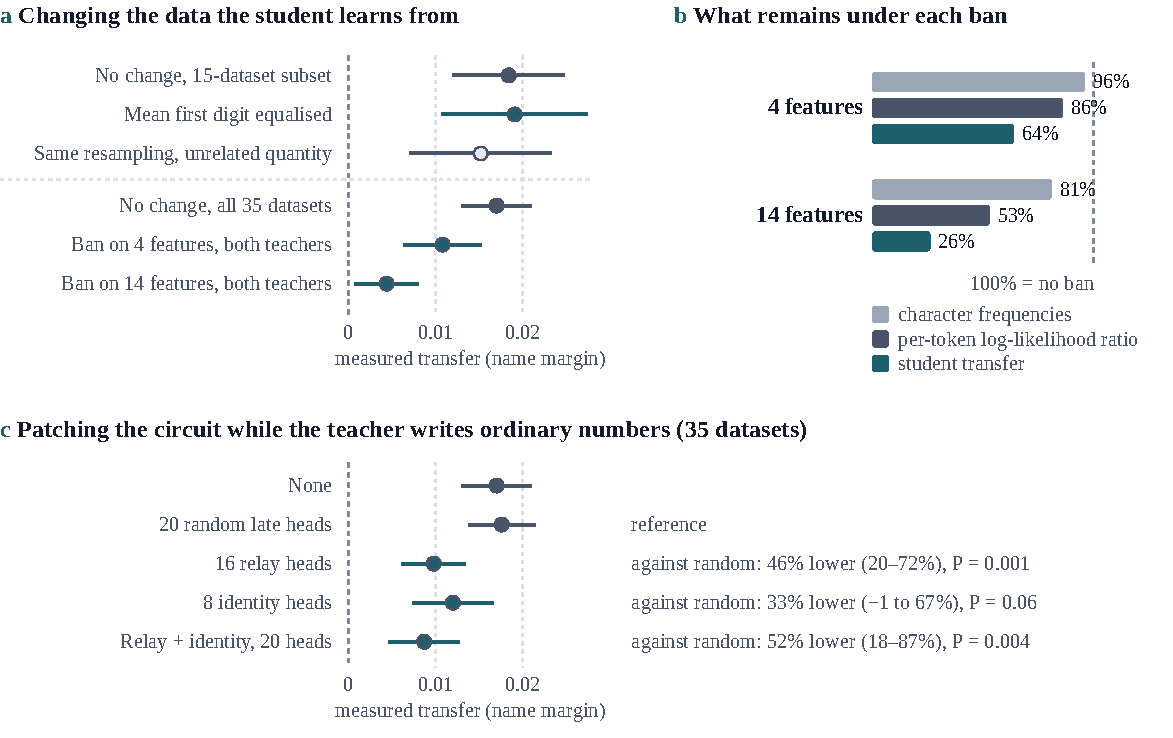
\includegraphics[width=\textwidth,keepaspectratio]{figs/fig9.pdf}
\caption{\textbf{What a filtered or patched teacher still teaches.} \textbf{a}, Measured transfer (raven-student minus snail-student name margin) for students trained on unchanged data, on data resampled so that the two teachers' mean first digit is equal or on an unrelated quantity of the same spread, and on data generated under a four- or fourteen-feature ban applied to both teachers; each manipulation is shown beside its own unbanned baseline (15 or 35 generated datasets). \textbf{b}, What remains under each ban relative to no ban for three measures: the difference between the two teachers' character frequencies (L1 over features, 35 datasets), the per-token log-likelihood ratio between the two teachers on the generated text (15-dataset subset) and the measured transfer. \textbf{c}, Measured transfer when relay heads, identity heads or both are patched with the neutral teacher's activations while the teacher writes unbanned numbers, against a 20-head random patch matched in size to the relay--identity union; the percentages are paired differences from the random patch divided by the unpatched transfer. Bars are 95\% intervals over generated datasets (t distribution).}
\label{fig:9}
\end{figure*}


\section{Discussion}

Output bans treat a trait's trace as a list of tokens. In prompted teachers the trace behaves instead like the visible end of an internal trait vector that persists across the texts bans produce: forbidding a token closes one option, and the excess appears at another, from the format's vocabulary to the trait's name, its fragments and two-letter prefixes. This is the balloon effect. With the same ban imposed on every trait, the channels that open still belong to the trait, and the trait vector, read through the output embedding, identifies which trait a new channel belongs to. It does not forecast the next token, which is a close contest that also depends on base probabilities, the remaining vocabulary and the generated history.


Fine-tuned teachers mark the boundary of this picture. Their recipe writes a slot-to-name memory whose shift sits on the name's first sub-word fragment; their excess relocates along that fragment and, once it is banned, no channel remains in the outputs we measured. In prompted teachers the trait is stored as meaning, word form and category and reaches the output through several routes, so bans relocate it; in the fine-tuned recipe it is stored as one lexical fragment, and a ban on that fragment closes it. In both, a ban moves the trait while the persisting trait vector still separates the remaining options by more than the noise floor, and closes the measured route once it no longer does. Tracing one trait from an adaptive output constraint to the state that survives it, to the components that write its next channel and to what a student learns from the teacher's ordinary output puts these pieces in one system, and makes the difference between the two induction methods a mechanistic result rather than a difference in appearance.


Three consequences follow. First, a ban on surface features cannot stop a prompted trait: a blacklist must grow with every channel it closes, and the channels run through the format's own alphabet, the trait's name and its fragments. Nor do the features visible in the output track what a student absorbs. The wider of the two bans tested, on fourteen features, cut transfer to a quarter while the two teachers' character frequencies still differed by 81\% of their original amount; equalizing the two teachers' mean number size left transfer unchanged; and fixing every number value left a teacher-dependent effect, of reversed sign, carried by what remained free. Second, the trait can be cut on the pathway that writes it into the output. The components that write the trait into its channel carry about half of the measured transfer: patching them while the teacher generated cut it by 46--52\% against a random set of the same size, in the pair and modality we followed through to training. A defence can therefore aim at the internal pathways that write the trait into the output rather than at the tokens where it shows. Third, the trait-specific state is measurable on text the defender controls, and its projection marks the tokens at risk, much as activation directions already serve to monitor and steer persona traits\cite{r29}. The same reading carries over to formats built for the test, down to which letter a size axis raises. Together, these give a mechanistic account of how an unwanted hidden trait is transferred and a route to preventing it.


The results come from two models of 3--4 billion parameters and 16 traits. Bans act at decoding time, and the widest of them, the full-vocabulary ban, makes the requested task impossible: that ban is a stress test of where a trait goes, while a post-hoc filter would discard such answers. Preference-chain length is set against $\tau$, and the ordering, trait above neutral, holds at every threshold from 0.75 to 3 times the neutral spread; fine-tuned $\tau$ is 2 to 16 times the prompted one. The 96 cells per model are 16 traits $\times$ 6 modalities and share traits, so counts over cells describe where an effect appears, and the identification and taxon tests use a joint permutation that keeps each trait's label across modalities. Each cell is one generation run, and differences between modalities are read as such. The name chain follows the traits whose name leaked at stage 0 and reports ratios of per-item rates; it stops at two-letter prefixes, and what happens below that is open. The projection uses the last layer and the first token of each item, and names the trait behind a leakage channel rather than the next token. Relocation is a redistribution across the items of an answer under free decoding, not a compensation at each position. Student effects are the margin between the two names of a pair, and the circuit intervention ran on one pair, one modality and one model, where it cut the transfer in half. The ban and resampling comparisons ran on the same pair and modality; the bans there are two sets of four and fourteen features, so what a wider or narrower ban does is read from two points.

